\begin{figure*}[tp]
    \centering
    % \vspace{3mm}
    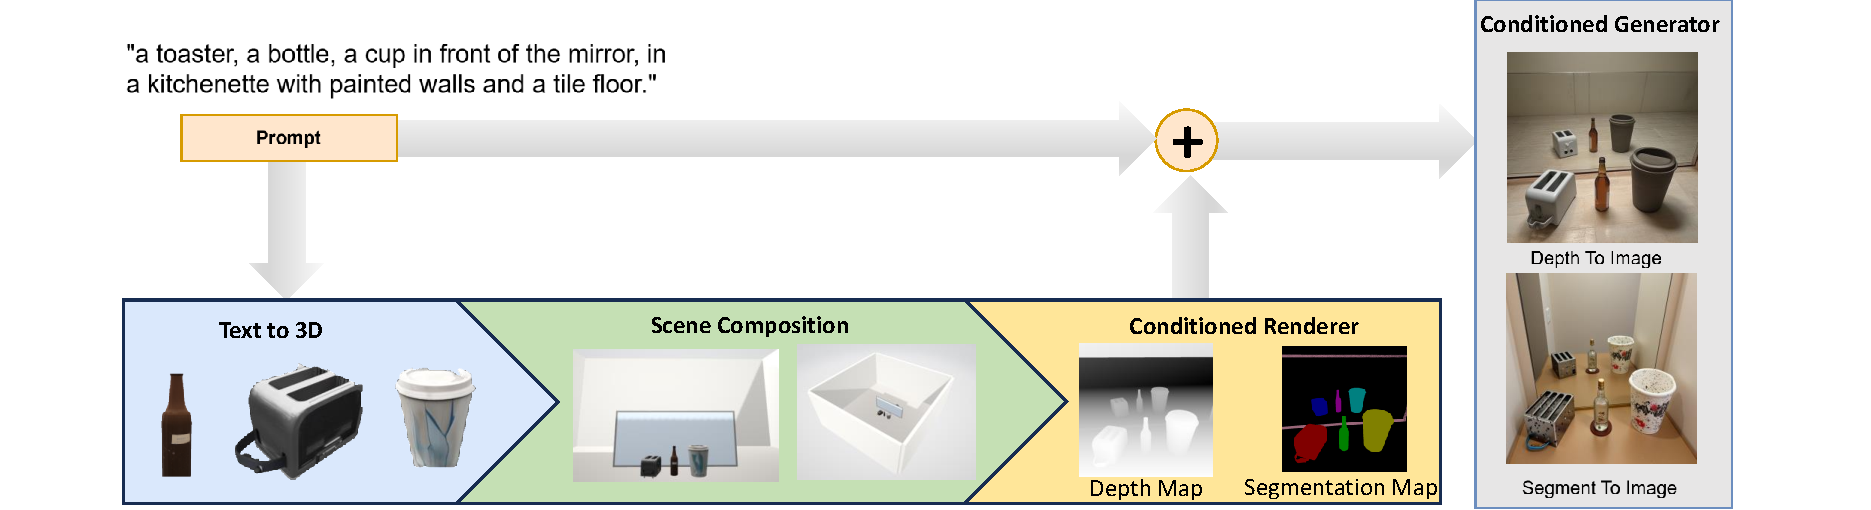
\includegraphics[width=\textwidth]{figures/proposed-method.pdf}
    \caption{Overview of the proposed PhysMirror. Given a text prompt, primary objects are parsed and lifted into 3D meshes via a text-to-3D model (Stage 1). These meshes are then assembled into a physically accurate 3D mirror scene (Stage 2). Next, a virtual camera is positioned to render precise spatial maps, such as depth and segmentation (Stage 3). Finally, these conditioning maps guide a text-to-image generative model to synthesize the final photorealistic image with geometrically correct mirror reflections (Stage 4).}
    \label{fig:proposed_method}
\end{figure*}